\chapter{Appendices}

\section{Appendix 1: Passing by Value and Reference}
\label{sec:appendix1}

This appendix provides three short, self-containted examples of ``na\"ive''
function hoisting in Rust. In each example, we will define a function that is
getting refactored, and we will demonstrate the case where the arguments to the
function are passed by value and the case where they are passed by reference. To
achieve this, we are imagining an automated refactoring tool that initially
takes an inline block of code and moves it into a new function. The compilation
errors (if any) guide a subsequent ownership analysis, which deduces how each
variable should be passed: by value (\texttt{T}), by shared reference
(\texttt{\&T}), or by mutable reference (\texttt{\&mut T}).

\subsection{Example 1: Passing by Value}
\subsubsection*{Original Code (inline)}
\inputminted{rust}{6_appendices/app1_code/ex1_oc.rs}

\subsubsection*{Na\"ive Hoisted Code (before fixes)}
Suppose an automated refactoring tool decides to “hoist” the multiplication
logic into a new function: \newline
\inputminted{rust}{6_appendices/app1_code/ex1_nhc.rs}
In this example, no errors occur because after calling
\texttt{hoisted\_block(x)}, we do not need \texttt{x} again in \texttt{main}, so
moving (passing ownership) is safe. The automated repair analysis detects that
\texttt{x} is no longer needed in \texttt{main} and decides it can be passed by
value.

\subsection{Example 2: Passing by Shared Reference}
\subsubsection*{Original Code (inline)}
\inputminted{rust}{6_appendices/app1_code/ex2_oc.rs}

\subsubsection*{Na\"ive Hoisted Code (before fixes)}
Let's say the refactoring tool decides to hoist the usage of \texttt{get\_first\_word} (or
a bit more logic around it) into a new helper function:
\inputminted{rust}{6_appendices/app1_code/ex2_nhc.rs}
This version won't compile as expected if the function
\texttt{print\_first\_word\_block} takes \texttt{text} by value. Once \texttt{text}
is moved into \texttt{print\_first\_word\_block}, we can no longer use
\texttt{text} afterward in \texttt{main}. The compiler will complain that
\texttt{text} is moved, thus invalidating the line \texttt{println!("Total
length is: {}", length);} if we needed \texttt{text} for anything else.

\subsubsection*{Automated Repair Yields}
\inputminted{rust}{6_appendices/app1_code/ex2_ar.rs}
\noindent What's going on?
\begin{itemize}
    \item \textbf{Read-only usage}: The function \texttt{print\_first\_word\_block}
    just needs to read the string (in order to print the first word).
    \item \textbf{Shared reference}: Because the string must remain valid
    afterward in \texttt{main}, the ownership analysis decides that passing by
    shared reference (\texttt{\&String}) is correct.
\end{itemize}

\subsection{Example 3: Passing by Mutable Reference}
\subsubsection*{Original Code (inline)}
\inputminted{rust}{6_appendices/app1_code/ex3_oc.rs}

\subsubsection*{Na\"ive Hoisted Code (before fixes)}
Hoisting the push operation into a new function could look like this:
\inputminted{rust}{6_appendices/app1_code/ex3_nhc.rs}
Here, we have a compilation error similar to Example 2: once \texttt{values} is
passed by value, ownership is transferred, and we cannot use \texttt{values}
again in \texttt{main}. However, in this case, we truly do need to mutate
\texttt{values}, and we want \texttt{main} to see the updated vector.

\subsubsection*{Automated Repair Yields}
\inputminted{rust}{6_appendices/app1_code/ex3_ar.rs}
\noindent What's going on?
\begin{itemize}
    \item \textbf{Mutation required}: The code needs to modify the original
    vector.
    \item \textbf{Mutable reference}: By passing \texttt{\&mut Vec<i32>}, the
    function can mutate \texttt{values} in place, and \texttt{main} retains
    ownership of \texttt{values} to use afterward.
\end{itemize}
 % Appendix 1 - Passing by Value and Reference
\newpage

\section{Appendix 2: Details of each Repository}
\label{sec:appendix2_details_of_each_repository}

\begin{table}[h]
\centering
\small

\begin{tabular}{|c|c|c|c|c|}
\hline
\textbf{Ranking} & \textbf{Project Repo}        & \textbf{Stars} & \textbf{Forks} & \textbf{Open Issues} \\ \hline
2  & denoland/deno                & 105077 & 5768  & 2384 \\
3  & rustdesk/rustdesk            & 102158 & 14993 & 61   \\
4  & tauri-apps/tauri             & 98717  & 3155  & 1161 \\
5  & unionlabs/union              & 74500  & 3835  & 155  \\
6  & astral-sh/uv                 & 72353  & 2212  & 2136 \\
7  & zed-industries/zed           & 69398  & 5885  & 3054 \\
8  & FuelLabs/sway                & 62106  & 5428  & 862  \\
9  & alacritty/alacritty          & 60977  & 3227  & 323  \\
10 & rust-lang/rustlings          & 60569  & 10978 & 46   \\
11 & FuelLabs/fuel-core           & 57463  & 2856  & 149  \\
12 & BurntSushi/ripgrep           & 57159  & 2304  & 85   \\
13 & topjohnwu/Magisk             & 56856  & 15853 & 36   \\
14 & sharkdp/bat                  & 55755  & 1409  & 318  \\
15 & meilisearch/meilisearch      & 54438  & 2254  & 221  \\
16 & lencx/ChatGPT                & 54214  & 6192  & 856  \\
17 & rust-unofficial/awesome-rust & 53670  & 3064  & 10   \\
18 & starship/starship            & 52113  & 2284  & 762  \\
19 & dani-garcia/vaultwarden      & 50694  & 2374  & 17   \\
20 & openai/codex                 & 50131  & 6215  & 1164 \\
21 & types/typst                  & 47876  & 1305  & 1007 \\ \hline
\end{tabular}

\captionsetup{justification=centering}
\caption{Brief summary of the 20 repositories searched to find real-world examples. \#1 is the Rust project itself.}
\label{tab:repo_summary}
\end{table}

\newpage

\begin{table}[h!]
\centering
\begin{tabular}{|c|p{3cm}|p{11cm}|}
\hline
\# & Name & URL \\ \hline

1  & denoland/\newline deno 
   & \url{https://github.com/denoland/deno/commit/104514b06dfbbb899235fb1147aa1fa62477a6d5} \\

2  & FuelLabs/\newline fuel-core
   & \url{https://github.com/FuelLabs/fuel-core/commit/ed92738280e068475682e220b93921bbbfebfdd7} \\

3  & meilisearch/\newline meilisearch
   & \url{https://github.com/meilisearch/meilisearch/commit/31142b36635ba062184b7d42f2e86021b11e911c} \\

4  & BurntSushi/\newline ripgrep
   & \url{https://github.com/BurntSushi/ripgrep/commit/7534d5144f5c5e89d67c791e663cdc0bee069b0e} \\

5  & starship/\newline starship
   & \url{https://github.com/starship/starship/commit/9093891acbe2c86b1615c37386dadbb0cc632199} \\

6  & FuelLabs/\newline sway
   & \url{https://github.com/FuelLabs/sway/commit/cdfc56c700ab32eefb84f75ed3048bd2a0ea22d2} \\

7  & tauri-apps/\newline tauri
   & \url{https://github.com/tauri-apps/tauri/commit/658e5f5d1dc1bd970ae572a42447448d064a7fee} \\

8  & unionlabs/\newline union
   & \url{https://github.com/unionlabs/union/commit/9b01ce6d75b84f049c1ede75750d33ce26ae73d9} \\

9  & astral-sh/\newline uv
   & \url{https://github.com/astral-sh/uv/commit/9af989e30c86391767830aa588c32fcb7c9a76b5} \\

10 & dani-garcia/\newline vaultwarden
   & \url{https://github.com/dani-garcia/vaultwarden/commit/952992c85bdf3147ddb8e663538e29c748b71f94} \\

11 & zed-industries/zed
   & \url{https://github.com/zed-industries/zed/commit/d00ad02b05981c79942b3bdff957e2384e68b89f} \\

\hline
\end{tabular}

\captionsetup{justification=centering}
\caption{Details of each repository in the evaluation, with the specific commit hash that we found examples from / evaluated against}
\label{tab:appendix2_details_of_each_repository}
\end{table}
 % Appendix 2 - Details of each Repository
\newpage 

\section{Appendix 3: GitOxide Example in Detail}
\label{sec:appendix_3}


The following diff shows how the `if add\_path` block was refactored into the
new helper method \texttt{extract\_include\_path}.

\begin{minted}[breaklines,fontsize=\small]{diff}
-        if add_path {
-            if let Some(body) = target_config.sections.get(&id) {
-                let paths = body.values(&Key::from("path"));
-                let paths = paths.iter().map(|path| values::Path::from(path.clone()));
-                include_paths.extend(paths);
-            }
-        }
         // Some specifics ommited for simplicity
+        if add_path {
+            extract_include_path(target_config, &mut include_paths, id)
+        }
\end{minted}

And here is the new method in full:

\begin{minted}[linenos,breaklines,fontsize=\small]{rust}
fn extract_include_path<'a>(
    target_config: &mut File<'a>,
    include_paths: &mut Vec<values::Path<'a>>,
    id: SectionId
) {
    if let Some(body) = target_config.sections.get(&id) {
        let paths = body.values(&Key::from("path"));
        let paths = paths.iter().map(|path| values::Path::from(path.clone()));
        include_paths.extend(paths);
    }
}
\end{minted} % Appendix 3 - GitOxide Example in more detail
\newpage

\section{Appendix 4: Complete MIR from \ref{content:subsec:charon}}

\inputminted[fontsize=\footnotesize,breaklines]{bash}{3_Chapter3/CHARON_example/mir_full.txt} % Appendix 4 - Complete MIR from rustc
\newpage 

\section{Appendix 5: Plotted Extraction time data}
\label{app:appendix5_extraction_histogram}

\begin{figure}[h!]
    \centering
    \includegraphics[width=\linewidth]{Figures/rem_extraction_time_breakdown.png}
    \caption{Execution time breakdown by pipeline stage for each test case.
    Times are reported in seconds (derived from nanosecond timing data).}
    \label{fig:rem_extraction_breakdown}
\end{figure}

\newpage

\begin{table}[h!]
\centering
\small
\begin{adjustwidth}{-1cm}{}
\begin{tabular}{|l|l|l|l|l|l|l|l|}
\hline
\multicolumn{1}{|c|}{Case} & \multicolumn{1}{c|}{\begin{tabular}[c]{@{}c@{}}Load the \\ Analysis\end{tabular}} & \multicolumn{1}{c|}{\begin{tabular}[c]{@{}c@{}}Analysis \\ Loaded\end{tabular}} & \multicolumn{1}{c|}{\begin{tabular}[c]{@{}c@{}}Get the \\ Assists\end{tabular}} & \multicolumn{1}{c|}{\begin{tabular}[c]{@{}c@{}}Filter For \\ EF Assist\end{tabular}} & \multicolumn{1}{c|}{\begin{tabular}[c]{@{}c@{}}Apply EF \\ Assist\end{tabular}} & \multicolumn{1}{c|}{Remaining} & \multicolumn{1}{c|}{Total} \\ \hline
beerus-ext-com1            & 9285                                                                              & 86226                                                                           & 2120                                                                            & 2060529                                                                                            & 2476                                                                                             & 5371                           & 2166007                    \\ \hline
gitoxide-ext-com1          & 307613                                                                            & 128739                                                                          & 2785                                                                            & 2887546                                                                                            & 2574                                                                                             & 7746                           & 3337003                    \\ \hline
gitoxide-ext-com2          & 10238                                                                             & 100897                                                                          & 2468                                                                            & 1872872                                                                                            & 2692                                                                                             & 28872                          & 2018039                    \\ \hline
gitoxide-ext1              & 454708                                                                            & 90926                                                                           & 2210                                                                            & 1583716                                                                                            & 3171                                                                                             & 13176                          & 2147907                    \\ \hline
gitoxide-ext2              & 468576                                                                            & 99266                                                                           & 2948                                                                            & 1449459                                                                                            & 3634                                                                                             & 6355                           & 2030238                    \\ \hline
gitoxide-ext3              & 593338                                                                            & 121557                                                                          & 2593                                                                            & 2098630                                                                                            & 4041                                                                                             & 30428                          & 2850587                    \\ \hline
gitoxide-ext4              & 387921                                                                            & 109024                                                                          & 2798                                                                            & 2715010                                                                                            & 3668                                                                                             & 21512                          & 3239933                    \\ \hline
gitoxide-ext5              & 520525                                                                            & 101651                                                                          & 2508                                                                            & 2183887                                                                                            & 2948                                                                                             & 11685                          & 2823204                    \\ \hline
gitoxide-ext6              & 529156                                                                            & 104946                                                                          & 2568                                                                            & 2342050                                                                                            & 2513                                                                                             & 10251                          & 2991484                    \\ \hline
gitoxide-ext7              & 290983                                                                            & 101383                                                                          & 2307                                                                            & 2869735                                                                                            & 5587                                                                                             & 11670                          & 3281665                    \\ \hline
gitoxide-inline-ext1       & 376787                                                                            & 96027                                                                           & 2954                                                                            & 2508828                                                                                            & 3532                                                                                             & 6906                           & 2995034                    \\ \hline
gitoxide-inline-ext2       & 496737                                                                            & 105101                                                                          & 2427                                                                            & 4729361                                                                                            & 3486                                                                                             & 8189                           & 5345301                    \\ \hline
gitoxide-inline-ext3       & 488481                                                                            & 122647                                                                          & 3248                                                                            & 4827718                                                                                            & 4000                                                                                             & 21855                          & 5467949                    \\ \hline
gitoxide-inline-ext4       & 495756                                                                            & 121965                                                                          & 3684                                                                            & 3281795                                                                                            & 5483                                                                                             & 15325                          & 3924008                    \\ \hline
gitoxide-inline-ext5       & 495051                                                                            & 112329                                                                          & 2474                                                                            & 2657133                                                                                            & 2991                                                                                             & 12808                          & 3282786                    \\ \hline
gitoxide-inline-ext6       & 622550                                                                            & 107609                                                                          & 2873                                                                            & 4480736                                                                                            & 3848                                                                                             & 22912                          & 5240528                    \\ \hline
gitoxide-inline-ext7       & 403207                                                                            & 96122                                                                           & 2356                                                                            & 2769977                                                                                            & 2617                                                                                             & 8734                           & 3283013                    \\ \hline
kickoff-ext1               & 494546                                                                            & 112377                                                                          & 3619                                                                            & 2768148                                                                                            & 2671                                                                                             & 14533                          & 3395894                    \\ \hline
kickoff-ext2               & 398752                                                                            & 124576                                                                          & 2850                                                                            & 2443569                                                                                            & 2733                                                                                             & 11091                          & 2983571                    \\ \hline
kickoff-ext3               & 492629                                                                            & 110374                                                                          & 2586                                                                            & 2531962                                                                                            & 2069                                                                                             & 13516                          & 3153136                    \\ \hline
kickoff-ext4               & 578567                                                                            & 108555                                                                          & 2736                                                                            & 2514134                                                                                            & 3164                                                                                             & 22551                          & 3229707                    \\ \hline
kickoff-inline-ext1        & 520277                                                                            & 126225                                                                          & 2583                                                                            & 2793580                                                                                            & 2920                                                                                             & 11691                          & 3457276                    \\ \hline
petgraph-ext1              & 374755                                                                            & 105993                                                                          & 2342                                                                            & 3306952                                                                                            & 3347                                                                                             & 9064                           & 3802453                    \\ \hline
petgraph-ext2              & 929776                                                                            & 181024                                                                          & 3519                                                                            & 7384406                                                                                            & 4936                                                                                             & 53650                          & 8557311                    \\ \hline
petgraph-ext3              & 881791                                                                            & 149205                                                                          & 2483                                                                            & 6287406                                                                                            & 2447                                                                                             & 42136                          & 7365468                    \\ \hline
petgraph-ext4              & 671999                                                                            & 123294                                                                          & 3069                                                                            & 4046105                                                                                            & 3188                                                                                             & 16542                          & 4864197                    \\ \hline
petgraph-ext5              & 400859                                                                            & 86750                                                                           & 2658                                                                            & 3688382                                                                                            & 3107                                                                                             & 9421                           & 4191177                    \\ \hline
petgraph-ext6              & 853792                                                                            & 154358                                                                          & 3156                                                                            & 6198179                                                                                            & 2902                                                                                             & 75377                          & 7287764                    \\ \hline
petgraph-inline-ext1       & 550082                                                                            & 114773                                                                          & 3004                                                                            & 4988262                                                                                            & 3287                                                                                             & 14740                          & 5674148                    \\ \hline
sniffnet-ext1              & 318576                                                                            & 89782                                                                           & 3191                                                                            & 4012997                                                                                            & 2925                                                                                             & 11313                          & 4438784                    \\ \hline
sniffnet-ext2              & 521024                                                                            & 108808                                                                          & 2324                                                                            & 2959298                                                                                            & 2719                                                                                             & 7431                           & 3601604                    \\ \hline
sniffnet-ext3              & 491132                                                                            & 114474                                                                          & 2420                                                                            & 2639553                                                                                            & 2501                                                                                             & 14870                          & 3264950                    \\ \hline
sniffnet-ext4              & 289206                                                                            & 104857                                                                          & 2458                                                                            & 3087829                                                                                            & 3184                                                                                             & 19270                          & 3506804                    \\ \hline
sniffnet-ext5              & 451829                                                                            & 112413                                                                          & 2904                                                                            & 3560519                                                                                            & 2571                                                                                             & 16898                          & 4147134                    \\ \hline
sniffnet-ext6              & 665962                                                                            & 163596                                                                          & 5027                                                                            & 3423886                                                                                            & 2428                                                                                             & 22809                          & 4283708                    \\ \hline
sniffnet-ext7              & 610395                                                                            & 115393                                                                          & 3062                                                                            & 3518957                                                                                            & 6090                                                                                             & 19601                          & 4273498                    \\ \hline
sniffnet-inline-ext1       & 606027                                                                            & 117642                                                                          & 2553                                                                            & 4392070                                                                                            & 8793                                                                                             & 30967                          & 5158052                    \\ \hline
sniffnet-inline-ext2       & 830359                                                                            & 110345                                                                          & 3269                                                                            & 1060569                                                                                            & 7246                                                                                             & 13375                          & 2025163                    \\ \hline
\end{tabular}
\captionsetup{justification=centering}
\caption{Raw timing data for the various extractions. Times are all in nanoseconds}
\end{adjustwidth}
\end{table}
\newpage 

\section{Appendix 6: (Almost) Complete Coq Translations}
\label{app:coq_translations}
Some of the Coq boilerplate has been removed to make these inclusions sensible. Still it is clear how massive the translation can get for even a small example. 

\captionsetup{justification=centering,type=listing}
\inputminted[
    fontsize=\scriptsize,
    linenos,
    frame=lines,
    breaklines
]{coq}{3_Chapter3/complex_example/Orig2.v}
\captionof{listing}{Original Coq translation, less some boilerplate}
\label{lst:orig-coq}

\newpage
\captionsetup{justification=centering,type=listing}
\inputminted[
    fontsize=\scriptsize,
    linenos,
    frame=lines,
    breaklines
]{coq}{3_Chapter3/complex_example/Wrong2.v}
\captionof{listing}{Coq translation of the Incorrect Extraction, less some boilerplate}
\label{lst:wrong-coq}
\newpage

\section{Appendix 7: New Extraction Feature Categories in Detail}
\label{app:new_extraction_features}

In this appendix we give concrete (although somewhat small) examples for each of the feature categories introduced in Section~\ref{subsec:new_language_features}. The examples are drawn from the repositories listed in Section~\ref{subsec:new_feature_cases}, or are lightly simplified variants of patterns we observed there, and are designed to isolate the behaviour of the extractor in the presence of a particular construct. In addition to asynchronous functions, const evaluation, generics, dynamic trait objects, and higher-ranked trait bounds, we include several instances of non-local control flow. Although the original REM toolchain could already handle some non-local control-flow refactorings, the new extraction engine implements them via the (now) standard \icodeverb{std::ops::ControlFlow} variants rather than custom enums, and we therefore evaluate them separately. Together, these examples characterise the kinds of advanced language mechanics that the original REM could not support and that the new toolchain is explicitly designed to handle, allowing us to check that it preserves semantics, typing, and compilation validity in each case.

\subsubsection{Generics (GEN)}

This case targets a generic function with multiple trait bounds, verifying that these are copied exactly to the extracted function. The extractor must not monomorphise or omit generic parameters, as doing so would restrict the function’s polymorphism and likely fail type checking. Additionally, if only a subset of the caller functions trait bounds apply to the callee (e.g. it only takes one of many generic arguments), then we would expect just the applicable trait bounds to be copied). 

\begin{minipage}[t]{0.43\linewidth}
    \vspace{0pt}% align tops
    \captionsetup{type=listing} 
    \inputminted[             fontsize=\scriptsize,             frame=lines,             linenos,             breaklines,         ]{rust}{6_appendices/app7_code/generics/before.rs}
    \captionof{listing}{Generics Example: Before}
    \label{lst:generics-before}
\end{minipage}
\hfill
\begin{minipage}[t]{0.43\linewidth}
    \vspace{0pt}
    \captionsetup{type=listing}
    \inputminted[             fontsize=\scriptsize,             frame=lines,             linenos,             breaklines,         ]{rust}{6_appendices/app7_code/generics/after.rs}
    \captionof{listing}{Generics Example: After}
    \label{lst:generics-after}
\end{minipage}

\subsubsection{Async and Await (ASYNC)}

This case targets extraction from within an \icodeverb{async fn}, where the inserted boundaries must remain within the compiler-generated state machine \footnote{\texttt{rustc} automatically generates a struct that acts as a state machine, with an internal state variable and a poll method. Each await point becomes a place where the state machine can pause, return \icodeverb{Poll::Pending}, and be resumed later by the runtime without losing its state.}.The extractor must correctly preserve the asynchronous context and the \icodeverb{Result} return type implied by \icodeverb{?}, while ensuring that lifetimes and borrows are not widened across the await suspension point. If the lifetimes produced by the extraction engine are incorrect, we expect REM-Repairer to correct them. 

\begin{minipage}[t]{0.43\linewidth}
    \vspace{0pt}% align tops
    \captionsetup{type=listing} 
    \inputminted[             fontsize=\scriptsize,             frame=lines,             linenos,             breaklines,         ]{rust}{6_appendices/app7_code/async/before.rs}
    \captionof{listing}{Async Example: Before}
    \label{lst:async-before}
\end{minipage}
\hfill
\begin{minipage}[t]{0.43\linewidth}
    \vspace{0pt}
    \captionsetup{type=listing}
    \label{lst:async-after}
    \inputminted[             fontsize=\scriptsize,             frame=lines,             linenos,             breaklines,         ]{rust}{6_appendices/app7_code/async/after.rs}
    \captionof{listing}{Async Example: After}
\end{minipage}

\subsubsection{Constant declarations (CONST)}

This case covers extraction within a \icodeverb{const fn}, which must remain evaluable at compile time under Rust's const-checking rules. Thus the extraction engine must identify const contexts, and where possible, propagate the \icodeverb{const} qualifier to the new function to maintain those guaruntees.

\begin{minipage}[t]{0.43\linewidth}
    \vspace{0pt}% align tops
    \captionsetup{type=listing} 
    \inputminted[             fontsize=\scriptsize,             frame=lines,             linenos,             breaklines,         ]{rust}{6_appendices/app7_code/const/before.rs}
    \captionof{listing}{CONST Example: Before}
    \label{lst:const-before}
\end{minipage}
\hfill
\begin{minipage}[t]{0.43\linewidth}
    \vspace{0pt}
    \captionsetup{type=listing}
    \inputminted[             fontsize=\scriptsize,             frame=lines,             linenos,             breaklines,         ]{rust}{6_appendices/app7_code/const/after.rs}
    \captionof{listing}{CONST Example: After}
    \label{lst:const-after}
\end{minipage}

\subsubsection{Non Local Control Flow (NLCF)}

This case covers all aspects of NLCF, being \icodeverb{return}, \icodeverb{break}, and \icodeverb{continue} in Rust. NLCF objects cannot cross function boundaries, and as such the extraction engine must reify control flow into a return value, using \icodeverb{std::ops::ControlFlow} variants to communicate termination or continuation back to the caller. As mentioned previously, this differs from REM's original insertion of custom enums to outline control flow handling, as we rely on the extraction engine to provide this information rather than REM-Controller. 

\begin{minipage}[t]{0.43\linewidth}
    \vspace{0pt}% align tops
    \captionsetup{type=listing} 
    \inputminted[             fontsize=\scriptsize,             frame=lines,             linenos,             breaklines,         ]{rust}{6_appendices/app7_code/NLCF/before.rs}
    \captionof{listing}{NLCF Example: Before}
    \label{lst:nlcf-before}
\end{minipage}
\hfill
\begin{minipage}[t]{0.43\linewidth}
    \vspace{0pt}
    \captionsetup{type=listing}
    \inputminted[             fontsize=\scriptsize,             frame=lines,             linenos,             breaklines,         ]{rust}{6_appendices/app7_code/NLCF/after.rs}
    \captionof{listing}{NLCF Example: After}
    \label{lst:nlcf-after}
\end{minipage}

\subsubsection{Higher Ranked Trait Bounds (HRTB)}

This case examines extraction from functions parameterised by higher-ranked trait bounds such as \icodeverb{for<'a> Fn(&'a T) -> &'a T}. These bounds are not inferred implicitly and must be explicitly copied to the new function signature to maintain lifetime correctness. Again, REM-Repairer is expected to be called here to either a) verify that the lifetimes are correct, and / or b) fix the incorrect lifetime bounds.

\begin{minipage}[t]{0.43\linewidth}
    \vspace{0pt}% align tops
    \captionsetup{type=listing} 
    \inputminted[             fontsize=\scriptsize,             frame=lines,             linenos,             breaklines,         ]{rust}{6_appendices/app7_code/HRTB/before.rs}
    \captionof{listing}{HRTB Example: Before}
    \label{lst:hrtb-before}
\end{minipage}
\hfill
\begin{minipage}[t]{0.43\linewidth}
    \vspace{0pt}
    \captionsetup{type=listing}
    \inputminted[             fontsize=\scriptsize,             frame=lines,             linenos,             breaklines,         ]{rust}{6_appendices/app7_code/HRTB/after.rs}
    \captionof{listing}{HRTB Example: After}
    \label{lst:hrtb-after}
\end{minipage}

\subsubsection{Dynamic Trait Objects (DTO)}

Here we isolate extraction involving a \icodeverb{&dyn Trait} parameter to test the extraction engines preservation of dynamic dispatch and object safety. The extractor must retain the trait object type and avoid replacing it with a generic bound, which would alter runtime behaviour. The category also includes cases where a function's arguments implement a trait, e.g. \icodeverb{fn ident(s: impl Into<String> -> ...}. 

\begin{minipage}[t]{0.43\linewidth}
    \vspace{0pt}% align tops
    \captionsetup{type=listing} 
    \inputminted[             fontsize=\scriptsize,             frame=lines,             linenos,             breaklines,         ]{rust}{6_appendices/app7_code/DTO/before.rs}
    \captionof{listing}{DTO Example: Before}
    \label{lst:dto-before}
\end{minipage}
\hfill
\begin{minipage}[t]{0.43\linewidth}
    \vspace{0pt}
    \captionsetup{type=listing}
    \inputminted[             fontsize=\scriptsize,             frame=lines,             linenos,             breaklines,         ]{rust}{6_appendices/app7_code/DTO/after.rs}
    \captionof{listing}{DTO Example: After}
    \label{lst:dto-after}
\end{minipage} % Appendix 7 - Extraction Feature Categories - moved from section 5.4.3 to make space in the body of the report.
\newpage 

\section{Appendix 8: Implementation of the Verification Pipeline}
\label{app:implementation_verification}

This appendix contains a much more thorough dive into all of the implementation details behind the equivalence proover. It is intended to be read alongside the source code, and will in places contain duplicate information from Section~\ref{sec:implementation_verification}.

\vspace{5mm}

\begin{minipage}[t]{0.55\textwidth}
\vspace{-90mm}
The design of REM2.0's equivalence checking is guided by two principles: (1)
verification must require no additional annotations or input from the developer,
and (2) it must complete quickly enough to fit into interactive IDE workflows.
To achieve this, the pipeline translates both the original program $P$ and the
refactored program $P'$ into progressively more structured semantic
representations, culminating in a machine-checked proof of observational
equivalence.

At a high level, the pipeline consists of five stages: \textbf{Extraction},
\textbf{REM repairs}, \textbf{CHARON translation}, \textbf{AENEAS
functionalisation}, and \textbf{Coq verification}. Each stage builds on the
previous one, gradually exposing the semantics of the refactored code, before we end up with the pure, functional model in Coq. Figure
\ref{fig:verification_pipeline} provides an overview of the entire process. We will only very briefly cover off on extraction and lifetime repairing in this section, please refer to Chapter \ref{chap:expanding_rem} for the full scope.
\end{minipage}
\hfill
\begin{minipage}[t]{0.35\textwidth}
\centering
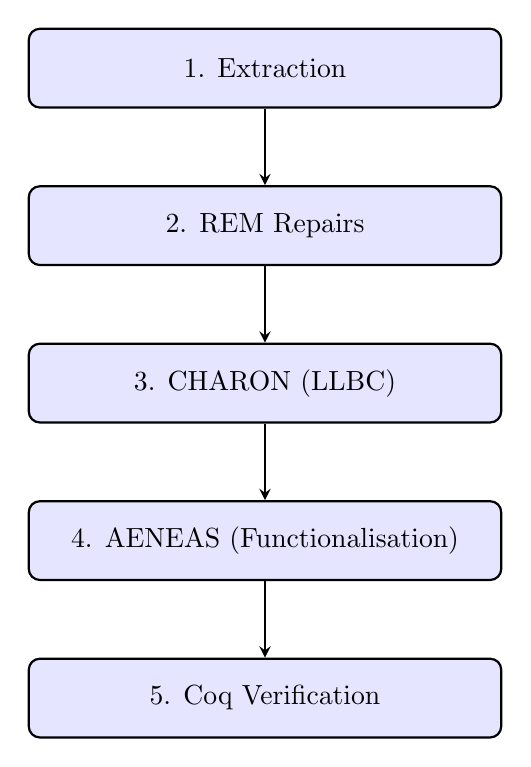
\begin{tikzpicture}[node distance=2cm, >=stealth, thick]
  % Nodes
  \node[draw, rounded corners, fill=blue!10, minimum width=6cm, minimum height=1cm] (extract) {1. Extraction};
  \node[draw, rounded corners, fill=blue!10, minimum width=6cm, minimum height=1cm, below of=extract] (rem) {2. REM Repairs};
  \node[draw, rounded corners, fill=blue!10, minimum width=6cm, minimum height=1cm, below of=rem] (charon) {3. CHARON (LLBC)};
  \node[draw, rounded corners, fill=blue!10, minimum width=6cm, minimum height=1cm, below of=charon] (aeneas) {4. AENEAS (Functionalisation)};
  \node[draw, rounded corners, fill=blue!10, minimum width=6cm, minimum height=1cm, below of=aeneas] (coq) {5. Coq Verification};

  % Arrows
  \draw[->] (extract) -- (rem);
  \draw[->] (rem) -- (charon);
  \draw[->] (charon) -- (aeneas);
  \draw[->] (aeneas) -- (coq);
\end{tikzpicture}

\captionof{figure}{Overview of the verification pipeline: from source code extraction to proof of observational equivalence in Coq.}
\label{fig:verification_pipeline}
\end{minipage}

\vspace{-2.5mm}
\subsection{Extraction}
Extraction lifts a user-selected region into a new function and replaces the selection with a call at the original site. As detailed in Section \ref{sec:single_file_workspace}, this step is powered by a Rust-Analyzer (RA) backed engine that performs single-file incremental analysis. It resolves the selection’s AST and symbol information in memory and synthesises a function skeleton together with the call-site edit.

The extraction result is returned as a deterministic set of edits (a patch) and a machine-readable summary for downstream stages. By design, the extractor does not attempt to finalise lifetimes or advanced ownership modes—that responsibility is delegated to REM’s repair phase. This separation keeps extraction millisecond fast and predictable, and completely independent of crate size, while ensuring a stable interface for the later verification.

\vspace{-2.5mm}
\subsection{REM}
REM performs \textit{post-extraction} semantic repair to attempt to bring the extracted code back into alignment with Rust's ownership and lifetime rules. Whilst much of the original REM toolchain's efforts have been integrated into the extraction process, we still rely heavily on the most complex part of REM's analysis: the Lifetime reification. We introduce, propagate, and constrain lifetime parameters to satisfy the borrow checker, generalising where necessary.

As detailed earlier, REM treats the compiler as an oracle: it iterates repairs until the program compiles, and then attempts to apply lifetime elision to produce a human-readable signature (where practical) and a function body that aligns as closely as possible to idiomatic Rust. The output of REM is thus the repaired program $P'$, which is then passed onto CHARON to begin the process of discharging equivalence obligations. 

\vspace{-2.5mm}
\subsection{CHARON}
\label{subsec:charon}

The first (new) stage of our verification pipeline is translation from Rust into a
lower-level, verification-friendly form. This role is performed by
\textbf{CHARON}, a Rust to LLBC (Low-Level Borrow Calculus) translator. CHARON
accepts Rust source code (or more precisely, its compiler intermediate
representation MIR) \footnote{Even more precisely, the tool itself accepts Rust
code, but its initial steps rely on a complex interaction with \texttt{rustc} to
acquire the MIR}. CHARON's main task is to extract complex semantic information
from \verb|rustc| and produce a machine readable output containing said
information. Up until this point, we have been working with / reasoning about a single file. Whilst this kept extraction lightning fast, CHARON's support for single file conversion is limited at best\footnote{CHARON can convert just a single file, but it relies on \texttt{rustc} to do so, and as such the single file must be self contained, which we cannot guarantee}. 

Thus at this stage, we construct two ``virtual'' crates within the users temporary directory (\icodeverb{std::env::temp()}). The advantages of this approach are:
\begin{enumerate}
    \item Any changes the user makes to their source code whilst we are performing the later stages of analysis will not get passed down to us (potentially introducing half written words or other bugs that would fail immediately)
    \item We do not require a file lock on the users code, so they can continue work
    \item We can safely abstract away the creation / deletion of the virtual crates, and have them live for only so long as the equivalence engine runs for, using a custom implementation of the \icodeverb{Drop} trait. 
    \item We can limit the data passing over the JSON-RPC bridge to just the original and extracted code for the file the user is working in. 
\end{enumerate}

CHARON then performs several non-trivial transformations:
\begin{itemize}
  \item \textbf{Structured control flow.}  
    MIR is a control-flow graph with arbitrary \icodeverb{goto}s; CHARON reconstructs
    this into structured \icodeverb{if}, \icodeverb{match}, and \icodeverb{loop} constructs,
    or preserves the raw form with the \texttt{--ullbc} option.

  \item \textbf{Trait and type resolution.}  
    Explicitly records how trait bounds are proven, normalises default methods,
    and can transform associated types into explicit parameters
    (\texttt{--remove-associated-types}).

  \item \textbf{Lifetime handling.}  
    Hides the distinction between early- and late-bound variables and makes
    implied bounds explicit, simplifying reasoning about generic functions.

  \item \textbf{Closures and vtables.}  
    Represented as ordinary structs implementing the relevant \texttt{Fn*}
    traits, making them accessible to later verification steps.

  \item \textbf{Noise reduction.}  
    Options such as \texttt{--hide-marker-traits} remove built-in traits
    (\icodeverb{Sized}, \icodeverb{Send}, etc.) that would otherwise clutter the output.
\end{itemize}

The result is a cleaned, semantically faithful program in LLBC form. Unlike raw
MIR, which is compiler-oriented, LLBC is designed for verification: ownership
and borrowing are represented directly, trait resolution is explicit, and
control flow is structured. A sample program and small portion of its MIR are
shown below. However, the output of CHARON is not designed for human
readability, and even the tiny program in Figure \ref{fig:charon_translation}
produces over 140,000 characters of LLBC. This (very verbose) explicitness is
what enables the subsequent translation into pure functional code for
verification.

\begin{figure}[ht]
  \small
  \centering
  \begin{minipage}[t]{0.45\linewidth}
    \inputminted[fontsize=\footnotesize]{rust}{3_Chapter3/CHARON_example/rust.rs}
    \vfill
    \captionsetup{type=listing}
    \caption{Rust source}
  \end{minipage}
  \hfill
  \begin{minipage}[t]{0.45\linewidth}
    \inputminted[fontsize=\footnotesize]{text}{3_Chapter3/CHARON_example/mir.txt}
    \vfill
    \captionsetup{type=listing}
    \caption{Excerpt of MIR (\texttt{rustc})}
  \end{minipage}
  \captionsetup{justification=centering}
  \caption{Illustration of CHARON's role. While only Rust and MIR are shown here, CHARON translates the MIR into LLBC. The LLBC is only designed to be machine readable, and as such is ommitted}
  \label{fig:charon_translation}
\end{figure}

\vspace{-2.5mm}
\subsection{AENEAS}
With the program translated into LLBC by CHARON, the next stage of the pipeline
is handled by \textbf{AENEAS}. AENEAS takes the borrow- and lifetime–explicit
LLBC and translates it into a \emph{purely functional form}, stripping away
low-level memory operations while preserving the program's semantics. This
functionalisation step is what makes the program suitable for downstream
reasoning in Coq: instead of reasoning about references and loans, we can reason
about values and functions. Currently AENEAS supports translation into
\emph{Coq, Lean, HOL4}, and \emph{F*}.

In practice, AENEAS acts as the bridge between compiler-level detail and
proof-level abstraction. CHARON ensures that all the complexities of lifetimes,
loads, and trait resolution are made explicit; AENEAS then packages these into a
form where correctness properties can be stated and proved without touching the
borrow checker or the stack/heap. Within the context of our pipeline, this is the point where Rust
code ``stops being Rust'' and becomes a functional program whose equivalence can
be checked in Coq.

\vspace{-2.5mm}
\subsection{Coq}
AENEAS translates the LLBC into a purely functional form, targeting Coq. The
final stage of the pipeline then combines the two generated Coq files ($P_{coq}$
and $P'_{coq}$), together with all auxiliary information needed to
automatically verify the equivalence between the original and refactored Rust
programs. A key challenge at this stage is the verbosity of the generated Coq
code (as illustrated in Listing~\ref{lst:complex-wrong-coq}), which led us to
implement a custom Coq tokeniser and parser tailored to the format emitted by
AENEAS.

In parallel with these translations, the equivalence prover’s main task is to
produce the \texttt{EquivCheck.v} file. This module instantiates both the
original and refactored definitions and generates an equivalence theorem, which
is a Coq encoding of the obligation(s) described in Section~\ref{sec:proof_obligations}. In practice, this means the Coq project is set up so that
it automatically checks that the two versions produce the same results for all
inputs. We defer the details of the proof obligations to that section; the key
point here is that the generated Coq project is self-contained: once compiled,
the equivalence is verified without further user intervention.

\vspace{-2.5mm}
\subsubsection*{What is Coq?}
Coq is an interactive theorem prover and proof assistant built on a dependently
typed functional language. It allows developers to define mathematical objects,
programs, and logical propositions, and to construct machine-checked proofs
about them. Every proof is validated by Coq's small, trusted kernel, giving very
high assurance of correctness. Coq has a long history of use in large-scale
verification projects—such as CompCert (a verified C compiler) and formally
verified operating systems—making it a natural fit for reasoning about the
safety and correctness of Rust programs.

\vspace{-2.5mm}
\subsubsection*{Why Coq?}
Coq was selected over alternatives such as HOL4, Lean, or F* for three main reasons:
\begin{itemize}[leftmargin=*,itemsep=0pt,topsep=2pt]
  \item \textbf{Mature ecosystem}  
    Decades of development have produced robust tooling, extensive libraries,
    and a stable kernel.

  \item \textbf{Direct integration}  
    AENEAS already targets Coq, whereas HOL4 and Lean would require substantial
    new backends for compatibility.

  \item \textbf{Automation}  
    Coq's tactic language and SMT integrations allow many routine proofs—
    such as equivalence checks—to be discharged automatically.
\end{itemize}

Lean and HOL4 both provide highly expressive grammars, but at the cost of
significant engineering effort to integrate with AENEAS \footnote{They both require even more additional supporting architecture on top of the current pipeline}. Whilst F* would require the least additional infrastructure, the platform is not that mature mature and would also duplicate existing
functionality. Coq therefore offers the best combination of maturity,
automation, and direct compatibility with our pipeline. % implementation of the verifyer in detail
\newpage

\section{Appendix 9: EquivCheck.v Lemmas from the Extraction Evaluation}
\label{app:lemmas}

\begin{figure}[h!]
    \centering
    \inputminted{coq}{6_appendices/app9_code/simple_lemma.txt}
    \captionof{listing}{EqivCheck.v file from one of the simple verification cases}
    \label{lst:lemma_example_simple}
\end{figure}

\begin{figure}[h!]
    \centering
    \inputminted[breaklines]{coq}{6_appendices/app9_code/complex_lemma.txt}
    \captionof{listing}{EqivCheck.v file from one of the complex verification cases}
    \label{lst:lemma_example_complex}
\end{figure} % Various equivalence stuff
